\documentclass[11pt,a4paper]{article}
\usepackage[margin=19mm]{geometry}
\usepackage[T1]{fontenc}
\usepackage{lmodern,microtype,graphicx,booktabs,array,tabularx,xcolor,tikz,titlesec,fancyhdr,hyperref}
\usetikzlibrary{arrows.meta,positioning,calc}
\definecolor{forest}{HTML}{214F36}
\definecolor{pale}{HTML}{F0F5EF}
\hypersetup{colorlinks=true,urlcolor=forest,linkcolor=forest,pdftitle={Rice Yield Prediction Preprocessing and Model Proposal},pdfauthor={R Ritwik and Joshith G}}
\titleformat{\section}{\centering\large\bfseries}{\thesection}{.6em}{}
\titleformat{\subsection}{\normalsize\bfseries}{}{0pt}{}
\titlespacing*{\section}{0pt}{8pt}{12pt}
\setlength{\parindent}{0pt}
\setlength{\parskip}{7pt}
\setlength{\emergencystretch}{2em}
\pagestyle{fancy}\fancyhf{}
\fancyfoot[L]{\footnotesize Rice yield preprocessing proposal}
\fancyfoot[R]{\footnotesize\thepage}
\renewcommand{\headrulewidth}{0pt}\renewcommand{\footrulewidth}{0pt}
\tikzset{box/.style={draw=forest,fill=pale,rounded corners=3pt,align=center,inner sep=8pt,font=\small},flow/.style={-{Stealth[length=2mm]},draw=forest,thick}}
\begin{document}

\begin{center}{\LARGE\bfseries Rice Yield Prediction\\[3pt] Preprocessing and Model Proposal}\end{center}
\begin{center}Faculty pitch for the South India rice yield project\end{center}
R Ritwik  |  23BAI0037\newline Joshith G  |  23BAI0075

\subsection*{Proposed project}
We propose to estimate district-level rice yield using crop statistics, location information and seasonal weather. We have assembled and preprocessed the data, including fitting a Denoising Autoencoder. The next stage is to train and compare yield predictors using conventional and learned input representations.

The central experiment is whether DAE feature learning improves yield prediction over standard preprocessing on the same observations. Improvement is a hypothesis to test, not an achieved result.

{\small\renewcommand{\arraystretch}{1.22}\setlength{\tabcolsep}{4pt}\begin{tabular}{>{\raggedright\arraybackslash}p{0.2724\linewidth}>{\raggedright\arraybackslash}p{0.6576\linewidth}}\toprule
\textbf{Scope} & \textbf{Current evidence}\\\midrule
Prediction target & Rice yield in tonnes per hectare\\[3pt]
Geographic coverage & Andhra Pradesh, Karnataka, Tamil Nadu and Telangana\\[3pt]
Observation unit & One district, crop year and season\\[3pt]
Merged data & 2,018 observations and 30 columns, covering 2001--2019\\[3pt]
Preprocessing & Standard transforms fitted; DAE fitted and outputs verified\\[3pt]
Prediction models & MLP and gradient-boosted trees proposed; not yet trained\\[3pt]
\bottomrule\end{tabular}}\par
\subsection*{Scope and reference paper}
Our selected reference is Paudel et al. (2023), Interpretability of deep learning models for crop yield forecasting. It forecasts European wheat and maize yield using LSTM and 1D CNN models. Our initial experiment adapts the yield task to Indian rice and seasonal tabular data; it is not an exact replication of that paper.

The present dataset has no disease labels or labelled crop images. We therefore do not claim disease diagnosis or nutrient-deficiency detection. Low predicted yield alone does not establish disease.

\clearpage\section*{Original data sources and the merge}
Three source families contribute to the master dataset. Previously separated yield, area and area-share tables were intermediate products of the same crop-statistics source, not additional independent raw datasets.

{\small\renewcommand{\arraystretch}{1.22}\setlength{\tabcolsep}{4pt}\begin{tabular}{>{\raggedright\arraybackslash}p{0.2126\linewidth}>{\raggedright\arraybackslash}p{0.3521\linewidth}>{\raggedright\arraybackslash}p{0.3654\linewidth}}\toprule
\textbf{Original source} & \textbf{Information supplied} & \textbf{Use in our dataset}\\\midrule
Government of India crop statistics & State, district, crop, year, season, cultivated area and production & Filter rice records; derive yield and area share\\[3pt]
GADM 4.1 district boundaries & Administrative district names and boundary coordinates & Match districts and attach representative longitude and latitude\\[3pt]
NASA POWER Daily API extract & Daily temperature, precipitation, wind, humidity, pressure, solar radiation and land evaporation & Aggregate district weather for each crop season\\[3pt]
\bottomrule\end{tabular}}\par
\begin{center}\resizebox{\linewidth}{!}{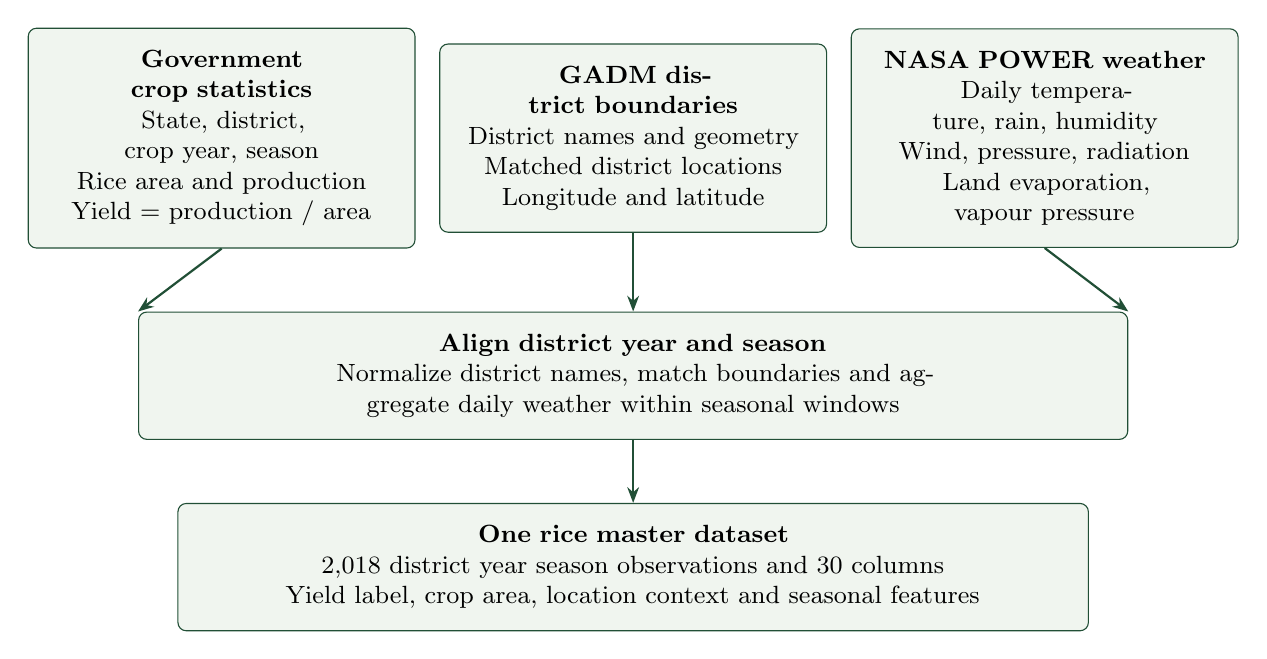
\begin{tikzpicture}
\node[box,text width=4.35cm] (a) {\textbf{Government crop statistics}\\State, district, crop year, season\\Rice area and production\\Yield = production / area};
\node[box,text width=4.35cm,right=3mm of a] (b) {\textbf{GADM district boundaries}\\District names and geometry\\Matched district locations\\Longitude and latitude};
\node[box,text width=4.35cm,right=3mm of b] (c) {\textbf{NASA POWER weather}\\Daily temperature, rain, humidity\\Wind, pressure, radiation\\Land evaporation, vapour pressure};
\node[box,text width=12cm,below=10mm of b] (j) {\textbf{Align district year and season}\\Normalize district names, match boundaries and aggregate daily weather within seasonal windows};
\node[box,text width=11cm,below=8mm of j] (m) {\textbf{One rice master dataset}\\2,018 district year season observations and 30 columns\\Yield label, crop area, location context and seasonal features};
\draw[flow] (a.south)--(j.north west);\draw[flow] (b)--(j);\draw[flow] (c.south)--(j.north east);\draw[flow] (j)--(m);
\end{tikzpicture}}\end{center}
{\footnotesize\itshape Figure 1  Three original source families become one aligned district year season table}\par
We normalize district names and match them to boundaries, using a historical state crosswalk where a unique match is available. Daily weather is aligned by district and seasonal dates. Rice area, production, derived yield and seasonal weather are then joined using the district identifier, crop year and season.

We retain records with matched locations, finite yield and at least 60 complete weather days. These conditions reduce 3,554 rice labels to 2,018 aligned observations. The retained data is source-derived; no simulated rows were added.

\clearpage\section*{Features in the merged rice dataset}
The master has 30 columns. Of these, 21 numerical features and two categorical fields are eligible predictor inputs. YIELD is the supervised label. Six remaining fields provide source context, identity or audit information.

{\small\renewcommand{\arraystretch}{1.22}\setlength{\tabcolsep}{4pt}\begin{tabular}{>{\raggedright\arraybackslash}p{0.186\linewidth}>{\raggedright\arraybackslash}p{0.3986\linewidth}>{\raggedright\arraybackslash}p{0.3454\linewidth}}\toprule
\textbf{Feature group} & \textbf{Columns} & \textbf{Meaning}\\\midrule
Crop area and location & CROP\_AREA, AREA\_FRACTION, CENTROID\_X, CENTROID\_Y & Rice area in hectares; district share of state-season rice area; longitude and latitude\\[3pt]
Weather coverage and temperature & WEATHER\_DAY\_COUNT, TMAX\_MEAN, TMIN\_MEAN, TAVG\_MEAN & Complete weather days and mean maximum, minimum and average temperatures in $^\circ$C\\[3pt]
Atmospheric conditions & VPRES\_MEAN, WSPD\_MEAN, RELH\_MEAN, PS\_MEAN & Mean vapour pressure, wind speed, relative humidity and surface pressure\\[3pt]
Seasonal totals & PREC\_TOTAL, ET0\_TOTAL, RAD\_TOTAL & Rainfall, land evaporation proxy and solar radiation accumulated over the season\\[3pt]
Derived numerical inputs & GDD\_BASE10, TEMP\_RANGE\_MEAN, WATER\_BALANCE\_PROXY, RAIN\_PER\_GDD, RADIATION\_PER\_GDD, CROP\_AREA\_LOG1P & Heat accumulation above 10$^\circ$C; temperature range; rain minus evaporation; weather totals per GDD; log-transformed area\\[3pt]
Categorical context & STATE, SEASON & Administrative state and crop season\\[3pt]
Target & YIELD & Reported production divided by rice area, in t/ha\\[3pt]
Not predictor inputs & CROP, IDREGION, DISTRICT, FYEAR, MATCH\_STATUS, PRODUCTION\_TONNES & Constant crop, record identity, split year, match audit and production\\[3pt]
\bottomrule\end{tabular}}\par
PRODUCTION\_TONNES is excluded because it directly determines YIELD together with area. Including it would leak the answer into the predictor. FYEAR is used for splitting, not as a current model input. The master retains these columns for provenance; exclusion does not mean deleting them from the source table.

Important interpretation: CENTROID\_X and CENTROID\_Y are averages of district boundary vertices, not area-weighted geographic centroids. ET0\_TOTAL retains a legacy column name but measures NASA EVLAND land evaporation, not FAO-56 reference evapotranspiration. RAD\_TOTAL is in kWh/m$^2$ for the selected NASA RE-community data.

\clearpage\section*{Preprocessing the merged dataset}
\begin{center}\resizebox{\linewidth}{!}{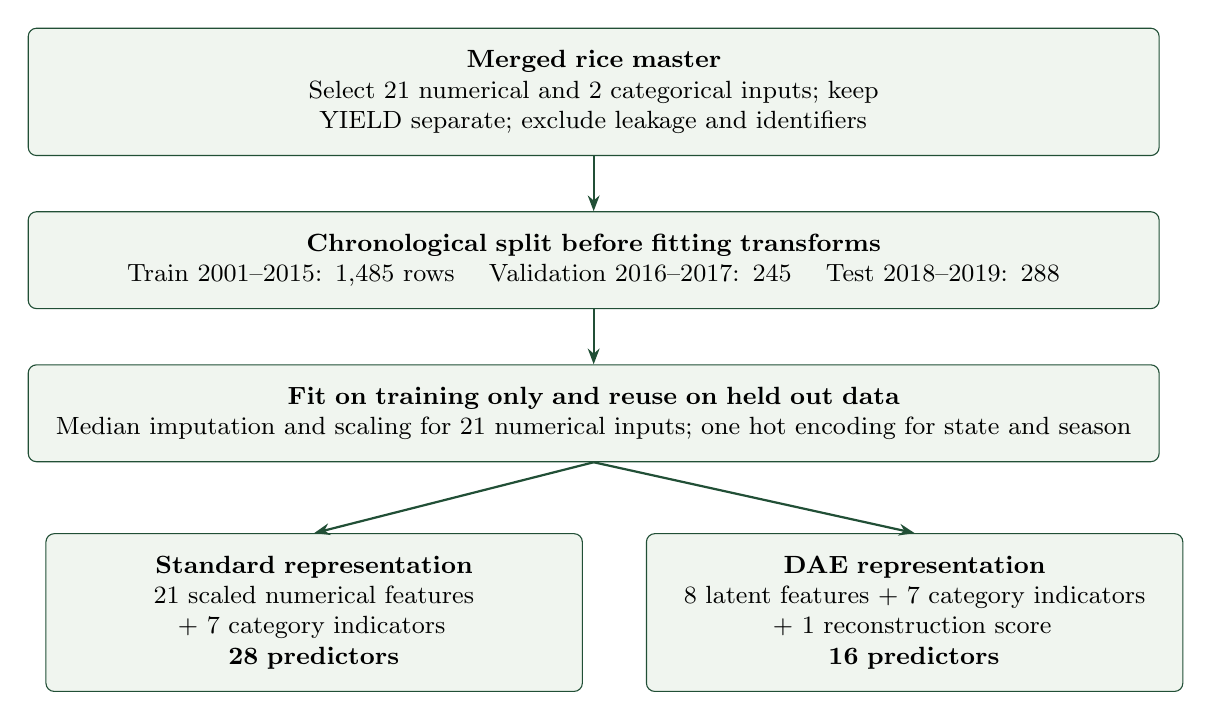
\begin{tikzpicture}
\node[box,text width=13.8cm] (a) {\textbf{Merged rice master}\\Select 21 numerical and 2 categorical inputs; keep YIELD separate; exclude leakage and identifiers};
\node[box,text width=13.8cm,below=7mm of a] (b) {\textbf{Chronological split before fitting transforms}\\Train 2001--2015: 1,485 rows \quad Validation 2016--2017: 245 \quad Test 2018--2019: 288};
\node[box,text width=13.8cm,below=7mm of b] (c) {\textbf{Fit on training only and reuse on held out data}\\Median imputation and scaling for 21 numerical inputs; one hot encoding for state and season};
\node[box,text width=6.25cm,below=9mm of c.south,xshift=-3.55cm] (s) {\textbf{Standard representation}\\21 scaled numerical features\\+ 7 category indicators\\\textbf{28 predictors}};
\node[box,text width=6.25cm,right=8mm of s] (d) {\textbf{DAE representation}\\8 latent features + 7 category indicators\\+ 1 reconstruction score\\\textbf{16 predictors}};
\draw[flow] (a)--(b);\draw[flow] (b)--(c);\draw[flow] (c.south)--(s.north);\draw[flow] (c.south)--(d.north);
\end{tikzpicture}}\end{center}
{\footnotesize\itshape Figure 2  Training-only preprocessing creates two comparable representations without changing labels}\par
\subsection*{Conventional transforms}
We split by year before learning transformation parameters. SimpleImputer learns numerical medians from training data; it is a safeguard for missing values even though the current master has none. StandardScaler uses training means and standard deviations to scale each numerical feature. OneHotEncoder turns STATE and SEASON into category indicators.

The fitted numerical and categorical transforms are reused on validation and test data without refitting. The standard output contains 21 scaled numerical predictors and seven category indicators, giving 28 predictors.

\subsection*{Learned preprocessing}
The DAE receives only the 21 standardized numerical inputs. During training, Gaussian noise with standard deviation 0.05 is added to the inputs, while the reconstruction target remains the clean standardized vector. The network learns to compress and reconstruct these inputs. State and season bypass the DAE and are encoded separately.

Its eight latent values are combined with seven category indicators and one per-row reconstruction MSE, giving 16 exported predictors. The reconstruction score is an optional auxiliary feature whose contribution should be evaluated separately. No yield labels are used to fit the DAE.

\clearpage\section*{What the preprocessing model learns}
\begin{center}\resizebox{\linewidth}{!}{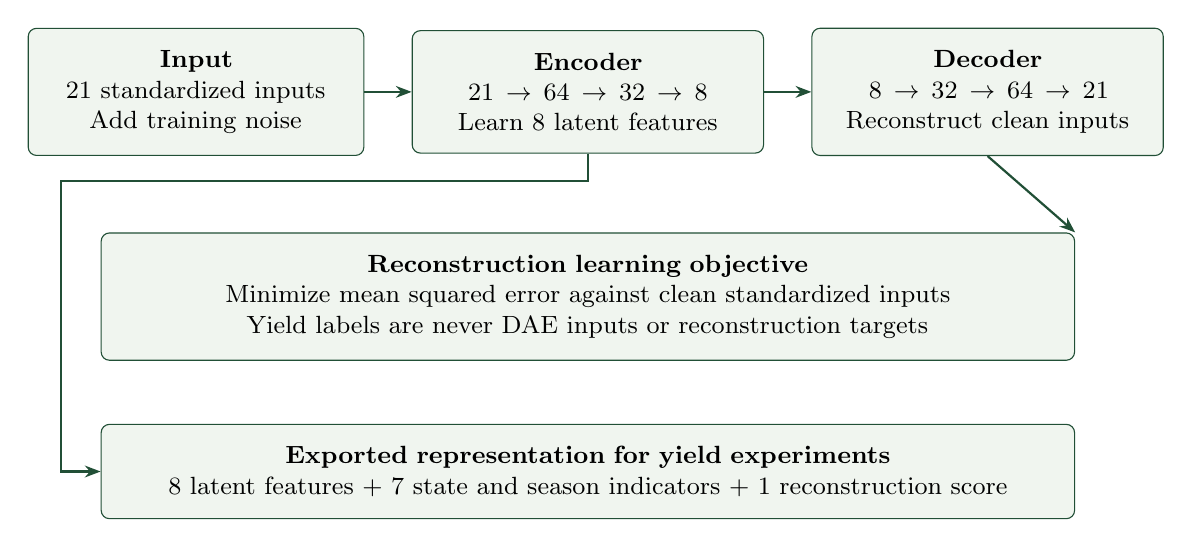
\begin{tikzpicture}
\node[box,text width=3.7cm] (i) {\textbf{Input}\\21 standardized inputs\\Add training noise};
\node[box,text width=3.9cm,right=6mm of i] (e) {\textbf{Encoder}\\$21\rightarrow64\rightarrow32\rightarrow8$\\Learn 8 latent features};
\node[box,text width=3.9cm,right=6mm of e] (d) {\textbf{Decoder}\\$8\rightarrow32\rightarrow64\rightarrow21$\\Reconstruct clean inputs};
\node[box,text width=11.8cm,below=10mm of e] (l) {\textbf{Reconstruction learning objective}\\Minimize mean squared error against clean standardized inputs\\Yield labels are never DAE inputs or reconstruction targets};
\node[box,text width=11.8cm,below=8mm of l] (o) {\textbf{Exported representation for yield experiments}\\8 latent features + 7 state and season indicators + 1 reconstruction score};
\draw[flow] (i)--(e);\draw[flow] (e)--(d);\draw[flow] (d.south)--(l.north east);\draw[flow] (e.south)--++(0,-.35cm)-|($(l.west)+(-.5cm,0)$)|-(o.west);
\end{tikzpicture}}\end{center}
{\footnotesize\itshape Figure 3  The DAE learns input representations rather than rice yield or disease labels}\par
The encoder learns eight numerical coordinates that jointly represent patterns in the 21 input features. These latent features do not each have a fixed meaning such as rainfall or temperature. The decoder is used to teach reconstruction; the learned encoder supplies the compact numerical inputs for the yield experiments.

{\small\renewcommand{\arraystretch}{1.22}\setlength{\tabcolsep}{4pt}\begin{tabular}{>{\raggedright\arraybackslash}p{0.2856\linewidth}>{\raggedright\arraybackslash}p{0.6444\linewidth}}\toprule
\textbf{DAE setting} & \textbf{Implemented choice}\\\midrule
Architecture & 21 $\rightarrow$ 64 $\rightarrow$ 32 $\rightarrow$ 8 $\rightarrow$ 32 $\rightarrow$ 64 $\rightarrow$ 21\\[3pt]
Layers and regularization & GELU activations; encoder BatchNorm; dropout 0.1\\[3pt]
Optimization & AdamW; learning rate 0.001; reconstruction MSE objective\\[3pt]
Run and checkpoint & 180 epochs completed; lowest validation MSE at epoch 178\\[3pt]
Measured validation result & Reconstruction MSE 0.07724 on standardized numerical inputs\\[3pt]
\bottomrule\end{tabular}}\par
\subsection*{What we have established}
The exported predictors are finite, the yield labels are preserved and the saved DAE checkpoint reproduces the exported latent features. These checks establish a working preprocessing pipeline. They do not establish higher yield accuracy, removal of real measurement errors or recovery of true field conditions.

This is an established Denoising Autoencoder approach adapted to our tabular inputs and fitted on our training split. It is not a pretrained agricultural model. The justification for using it is to test learned compression and resistance to injected perturbations, rather than to claim the assembled data needs no preprocessing.

\clearpage\section*{Merged data and preprocessed data compared}
{\small\renewcommand{\arraystretch}{1.22}\setlength{\tabcolsep}{4pt}\begin{tabular}{>{\raggedright\arraybackslash}p{0.1661\linewidth}>{\raggedright\arraybackslash}p{0.2458\linewidth}>{\raggedright\arraybackslash}p{0.2591\linewidth}>{\raggedright\arraybackslash}p{0.2591\linewidth}}\toprule
\textbf{Property} & \textbf{Merged master} & \textbf{Standard version} & \textbf{DAE version}\\\midrule
Observations & 2,018 total & Same 2,018, split by year & Same 2,018, split by year\\[3pt]
Numerical representation & 21 inputs in original or derived units & 21 scaled numerical features & 8 learned latent features\\[3pt]
State and season & Two text fields & 7 category indicators & 7 category indicators\\[3pt]
Additional predictor & None & None & 1 reconstruction MSE\\[3pt]
Predictor count & 23 eligible input fields before encoding & 28 numerical predictors & 16 numerical predictors\\[3pt]
Yield label & YIELD in t/ha & Same YIELD in t/ha & Same YIELD in t/ha\\[3pt]
Stored column count & 30 & 34: 28 predictors + label + 5 metadata & 22: 16 predictors + label + 5 metadata\\[3pt]
Purpose & Source traceability and dataset inspection & Conventional-feature yield experiments & Learned-feature yield experiments\\[3pt]
\bottomrule\end{tabular}}\par
The two preprocessed versions are alternative views of the same records. They are not separate populations, newly generated crop observations or extra training samples. The raw downloads and merged master remain unchanged; preprocessing creates new outputs.

{\small\renewcommand{\arraystretch}{1.22}\setlength{\tabcolsep}{4pt}\begin{tabular}{>{\raggedright\arraybackslash}p{0.1594\linewidth}>{\raggedright\arraybackslash}p{0.1993\linewidth}>{\raggedright\arraybackslash}p{0.1661\linewidth}>{\raggedright\arraybackslash}p{0.4052\linewidth}}\toprule
\textbf{Partition} & \textbf{Years} & \textbf{Observations} & \textbf{Purpose}\\\midrule
Training & 2001--2015 & 1,485 & Fit transforms, DAE and future yield predictors\\[3pt]
Validation & 2016--2017 & 245 & Select DAE checkpoint and yield-model settings\\[3pt]
Test & 2018--2019 & 288 & Final held-out yield evaluation\\[3pt]
\bottomrule\end{tabular}}\par
\subsection*{What dataset inspection revealed}
The master has no missing cells and no duplicate district year season keys. Coverage is uneven: Karnataka contributes 722 rows, Tamil Nadu 612, Andhra Pradesh 572 and Telangana 112. This supports reporting state-specific results rather than relying only on a pooled score.

Autumn and Winter are absent from the training years. Their season indicators currently become all zeros when transforming validation or test records. This limitation must be reported, and results for these seasons should be evaluated separately.

\clearpage\section*{Model roles and current status}
The first three methods are preprocessing tools, not neural networks. The DAE is the fitted preprocessing neural network. MLP and gradient-boosted trees are the proposed yield predictors for the initial tabular experiment.

{\small\renewcommand{\arraystretch}{1.22}\setlength{\tabcolsep}{4pt}\begin{tabular}{>{\raggedright\arraybackslash}p{0.2724\linewidth}>{\raggedright\arraybackslash}p{0.4849\linewidth}>{\raggedright\arraybackslash}p{0.1727\linewidth}}\toprule
\textbf{Model or method} & \textbf{Role in our project} & \textbf{Current status}\\\midrule
SimpleImputer & Fills missing numerical values using training-data medians & Fitted\\[3pt]
StandardScaler & Places numerical features on comparable scales using training statistics & Fitted\\[3pt]
OneHotEncoder & Converts state and season into numerical category indicators & Fitted\\[3pt]
Denoising Autoencoder\newline DAE & Compresses 21 numerical inputs into 8 latent features by reconstructing clean inputs from noisy versions & Trained\\[3pt]
Multilayer Perceptron\newline MLP regressor & Learns relationships between input features and rice yield; outputs predicted tonnes per hectare & Defined, not trained\\[3pt]
HistGradient\allowbreak Boosting\allowbreak Regressor & Predicts yield using boosted decision trees; provides a non-DL comparison & Defined, not trained\\[3pt]
Long Short Term Memory\newline LSTM regressor & Learns dependencies across weather time steps for yield prediction & Future sequence experiment\\[3pt]
One dimensional CNN\newline 1D CNN regressor & Learns local patterns across weather sequences for yield prediction & Future sequence experiment\\[3pt]
\bottomrule\end{tabular}}\par
\subsection*{How these roles differ}
The DAE learns to represent the inputs. MLP and gradient-boosted trees learn to predict YIELD from those representations. The encoder supplies the latent features; the decoder is also needed if we retain the reconstruction-score predictor. We compare both input versions rather than selecting the DAE version in advance.

LSTM and 1D CNN are the reference paper's deep-learning model families. They require explicit temporal sequences. Our present master contains seasonal summaries, so weather-sequence preparation is a later stage, not a completed part of the current experiment.

\clearpage\section*{Proposed experiments and faculty pitch}
\begin{center}\resizebox{\linewidth}{!}{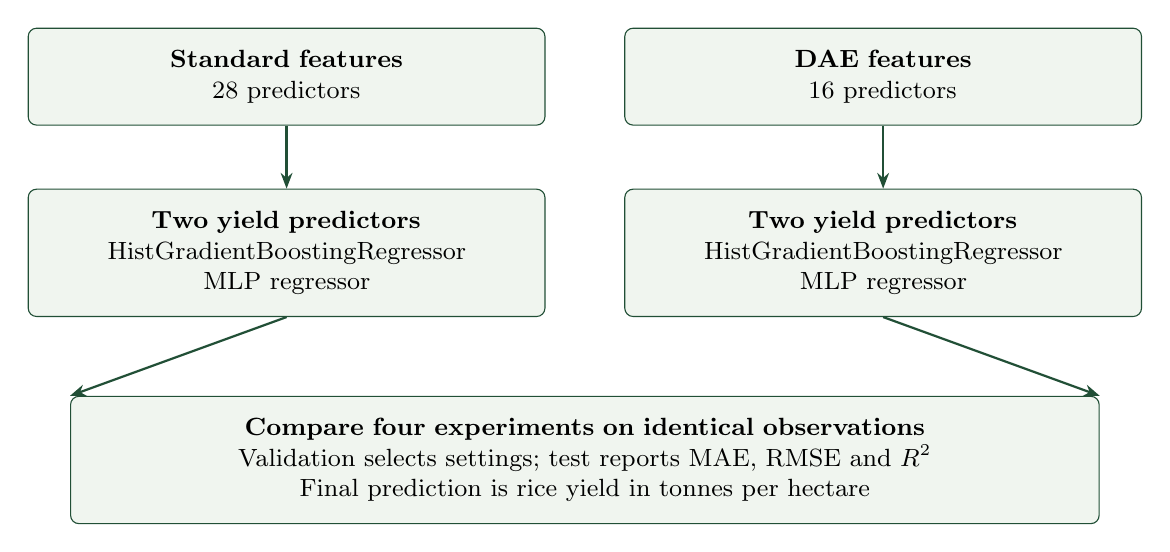
\begin{tikzpicture}
\node[box,text width=6cm] (s) {\textbf{Standard features}\\28 predictors};
\node[box,text width=6cm,right=10mm of s] (d) {\textbf{DAE features}\\16 predictors};
\node[box,text width=6cm,below=8mm of s] (m) {\textbf{Two yield predictors}\\HistGradientBoostingRegressor\\MLP regressor};
\node[box,text width=6cm,below=8mm of d] (n) {\textbf{Two yield predictors}\\HistGradientBoostingRegressor\\MLP regressor};
\node[box,text width=12.5cm,below=10mm of $(m.south)!.5!(n.south)$] (t) {\textbf{Compare four experiments on identical observations}\\Validation selects settings; test reports MAE, RMSE and $R^2$\\Final prediction is rice yield in tonnes per hectare};
\draw[flow] (s)--(m);\draw[flow] (d)--(n);\draw[flow] (m.south)--(t.north west);\draw[flow] (n.south)--(t.north east);
\end{tikzpicture}}\end{center}
{\footnotesize\itshape Figure 4  Four supervised experiments test the preprocessing choice and predictor choice}\par
{\small\renewcommand{\arraystretch}{1.22}\setlength{\tabcolsep}{4pt}\begin{tabular}{>{\raggedright\arraybackslash}p{0.1196\linewidth}>{\raggedright\arraybackslash}p{0.4251\linewidth}>{\raggedright\arraybackslash}p{0.3853\linewidth}}\toprule
\textbf{Experiment} & \textbf{Input representation} & \textbf{Yield predictor}\\\midrule
1 & Standard predictors & HistGradient\allowbreak Boosting\allowbreak Regressor\\[3pt]
2 & Standard predictors & MLP regressor\\[3pt]
3 & DAE predictors with encoded categories & HistGradient\allowbreak Boosting\allowbreak Regressor\\[3pt]
4 & DAE predictors with encoded categories & MLP regressor\\[3pt]
\bottomrule\end{tabular}}\par
We will use identical splits and labels, tune settings on validation data, then report test MAE, RMSE and R$^2$, with state and season breakdowns. Repeated neural-network seeds and an additional comparison without the reconstruction-score feature will help assess stability and the source of any improvement.

With 1,485 training rows, compact models and regularization are appropriate. Repeated records from the same districts are related. Claims will apply to the evaluated regions and years, not all of India or superiority over a European study using different inputs.

Our current full-season summaries support retrospective yield estimation. Forecasting before harvest requires rebuilding features using only information available at the forecast date. A future application would obtain location and weather context for user-selected district, season and year, then output predicted yield in t/ha; it will not diagnose disease.

\subsection*{Pitch summary}
We have combined three source families into a verified rice dataset for four South Indian states. We have fitted both standard transforms and a Denoising Autoencoder. We propose a controlled comparison of standard and learned features using an MLP and boosted trees, to determine whether neural-network preprocessing improves held-out yield estimation.

\clearpage\section*{Models used for supervised training}
Our initial supervised training uses two exact model types: \textbf{Multilayer Perceptron regressor (MLP)} and \textbf{HistGradientBoostingRegressor}. Each will be fitted separately on the standard and DAE representations, producing four experiments. LSTM and 1D CNN are later sequence-based extensions, not additional models already trained on these tables.

\subsection*{Training inputs and target}
The standard model receives a vector of 28 predictors: 21 scaled numerical features and seven encoded state and season indicators. The DAE-based model receives 16 predictors: eight learned numerical features, seven encoded indicators and one reconstruction score. For the score ablation, this becomes 15 predictors.

Each row has one supervised target, YIELD in tonnes per hectare. Training inputs exclude YIELD, production, raw district identifiers and split metadata. The target remains in physical units; the fitted input transforms must be reused consistently at prediction time. Only the 1,485 training observations fit yield-model parameters. Validation and test observations are not added to this fitting stage.

\subsection*{Multilayer Perceptron regressor}
An MLP is a feed-forward neural network for tabular inputs. Our defined architecture is:
\begin{center}
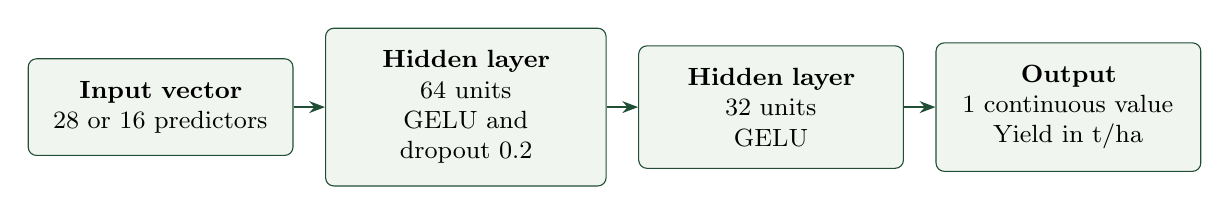
\begin{tikzpicture}
\node[box,text width=2.8cm] (a) {\textbf{Input vector}\\28 or 16 predictors};
\node[box,text width=3.0cm,right=4mm of a] (b) {\textbf{Hidden layer}\\64 units\\GELU and dropout 0.2};
\node[box,text width=2.8cm,right=4mm of b] (c) {\textbf{Hidden layer}\\32 units\\GELU};
\node[box,text width=2.8cm,right=4mm of c] (d) {\textbf{Output}\\1 continuous value\\Yield in t/ha};
\draw[flow] (a)--(b);\draw[flow] (b)--(c);\draw[flow] (c)--(d);
\end{tikzpicture}
\end{center}
{\footnotesize\itshape Figure 5  The same MLP structure accepts either preprocessing representation}\par
The network learns nonlinear combinations of crop area, weather and location context that help estimate yield. Backpropagation adjusts its weights using errors against observed YIELD. The output is a regression value, not a disease class or probability. A linear output can produce implausible values; we must check and report such cases rather than silently altering evaluation results.

\subsection*{Histogram gradient boosted trees}
HistGradientBoostingRegressor builds an additive ensemble of decision trees. Successive boosting steps reduce the current prediction error. It captures thresholds and interactions in the numerical predictors without requiring a neural network and supplies the comparison needed to assess whether DL is useful for this dataset.

The existing model factory defines an initial configuration of 200 boosting iterations, at most 15 leaves per tree, learning rate 0.05 and random seed 42. Its internal early stopping is disabled, so the explicit chronological validation split will guide selection of settings. These are starting settings, not validated optimal values.

\textbf{Current status.} Both supervised architectures are defined but have no fitted yield weights. Only the preprocessing transforms and DAE have been fitted. No supervised yield accuracy is available yet.

\clearpage\section*{Learning objectives and evaluation protocol}
\subsection*{Two different learning tasks}
The DAE learns an input representation without yield supervision. It reconstructs a clean standardized vector from a corrupted version. The proposed MLP instead uses YIELD supervision to estimate the observed yield. These objectives must not be treated as interchangeable measures of model quality.
\begin{center}
\begin{tabular}{p{.23\linewidth}p{.32\linewidth}p{.34\linewidth}}
\toprule
\textbf{Training stage} & \textbf{Learning signal} & \textbf{What is learned}\\\midrule
DAE preprocessing & Clean standardized inputs & A compact numerical representation and reconstruction\\[4pt]
MLP yield training & Observed yield label & Neural-network weights mapping predictors to yield\\[4pt]
Boosted tree training & Observed yield label & Tree splits and contributions mapping predictors to yield\\
\bottomrule
\end{tabular}
\end{center}
\subsection*{Proposed neural network training procedure}
We propose MSE loss for yield regression and AdamW optimization for the MLP, with small batches, regularization and checkpoint selection based on the chronological validation set. Learning rate, batch size, weight decay and epoch limit will be selected through a documented validation search. These are proposed training procedures, not settings already executed for yield prediction.

The fitted DAE remains frozen in the initial comparisons. Any later fine-tuning using yield labels must be evaluated as a separate experiment.

Repeated MLP runs will assess initialization sensitivity. We will record settings, seed, selected epoch and validation score. The test set remains untouched until the experiment configuration is fixed and must not guide selection.

\subsection*{Reported prediction metrics}
For $n$ held-out observations with true yield $y_i$ and predicted yield $\hat y_i$, we will report:
\[
\mathrm{MAE}=\frac{1}{n}\sum_{i=1}^{n}|y_i-\hat y_i|,
\qquad
\mathrm{RMSE}=\sqrt{\frac{1}{n}\sum_{i=1}^{n}(y_i-\hat y_i)^2}.
\]
MAE describes typical absolute error; RMSE puts greater weight on large errors. Both are in tonnes per hectare. $R^2$ describes performance relative to predicting the test-set mean and can be negative when a model performs poorly. Results will include predicted-versus-observed plots, residuals and state and season breakdowns.

\subsection*{What would count as improvement}
We will compare standard and DAE inputs within each predictor family on the same held-out observations. Lower yield error with stable repeated-run results would support using DAE preprocessing. If the DAE worsens prediction, that is evidence to prefer the standard representation. A low reconstruction MSE alone cannot support either conclusion.

We will separately examine the reconstruction-score ablation and the Autumn and Winter records that have unseen training categories. Temporal holdout measures later-year performance within the covered regions; it does not establish generalization to unseen states or districts. Reference-paper results cannot be directly ranked against ours because the crops, regions and available inputs differ.

\clearpage\section*{Future sequence models and application flow}
\subsection*{Long Short Term Memory regressor}
The defined LSTM accepts a weather sequence with ten weather channels per time step, its true sequence length and separate static or contextual inputs. It uses two recurrent layers with 64 hidden units and dropout 0.2. The last hidden representation is joined with context, then passed through a 64-unit GELU head with dropout 0.2 and a single yield output.

It can learn dependencies across weather time steps. Temporal sequence preparation, forecast cutoffs and train-only transforms are still required; these are not the current seasonal tables.

\subsection*{One dimensional Convolutional Neural Network regressor}
The defined 1D CNN takes ten weather channels across a fixed temporal window. Two convolution layers use 32 then 64 channels, kernel size three and GELU activations. Global average pooling creates a 64-value weather summary; context is appended and a 64-unit head with dropout 0.2 outputs yield.

It learns local temporal patterns and expects fixed-length unpadded sequences. Sequence preparation and training remain future work. Both sequence definitions are paper-inspired, not verified reproductions of its tuned configurations.

\subsection*{Proposed prediction workflow}
\begin{center}\resizebox{.85\linewidth}{!}{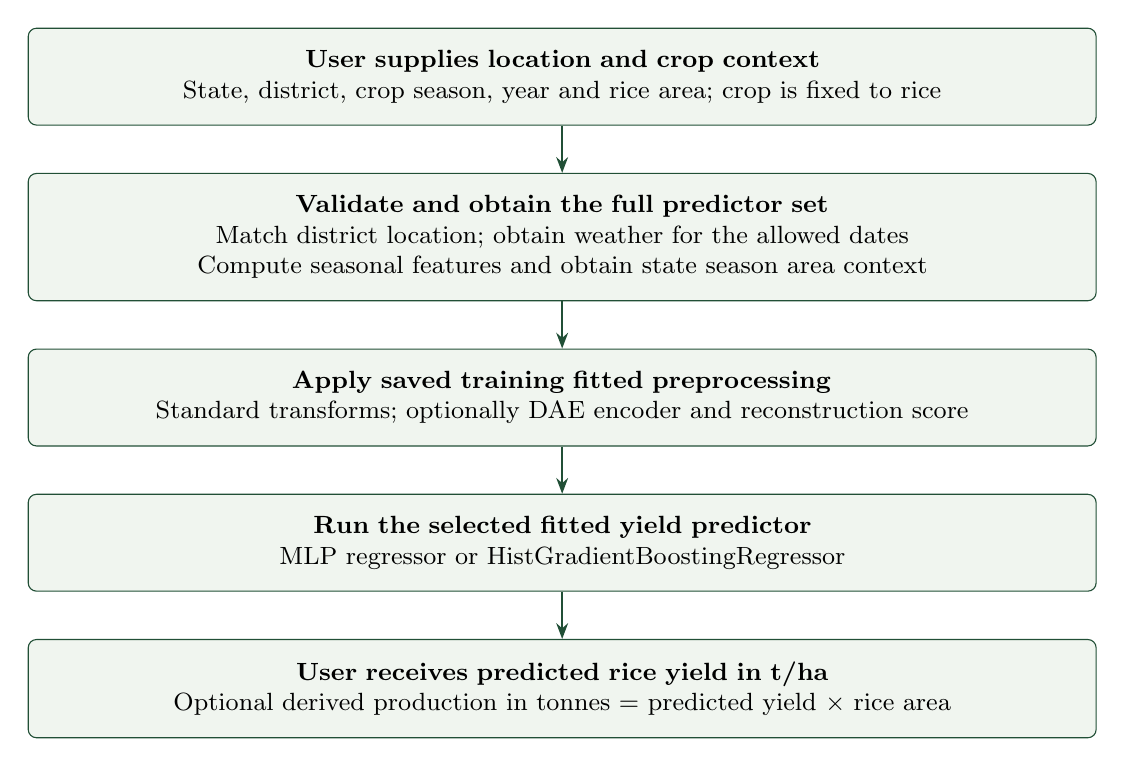
\begin{tikzpicture}
\node[box,text width=13cm] (u) {\textbf{User supplies location and crop context}\\State, district, crop season, year and rice area; crop is fixed to rice};
\node[box,text width=13cm,below=6mm of u] (f) {\textbf{Validate and obtain the full predictor set}\\Match district location; obtain weather for the allowed dates\\Compute seasonal features and obtain state season area context};
\node[box,text width=13cm,below=6mm of f] (p) {\textbf{Apply saved training fitted preprocessing}\\Standard transforms; optionally DAE encoder and reconstruction score};
\node[box,text width=13cm,below=6mm of p] (m) {\textbf{Run the selected fitted yield predictor}\\MLP regressor or HistGradientBoostingRegressor};
\node[box,text width=13cm,below=6mm of m] (o) {\textbf{User receives predicted rice yield in t/ha}\\Optional derived production in tonnes = predicted yield $\times$ rice area};
\draw[flow] (u)--(f);\draw[flow] (f)--(p);\draw[flow] (p)--(m);\draw[flow] (m)--(o);
\end{tikzpicture}}\end{center}
{\footnotesize\itshape Figure 6  Proposed inference requires weather and area context in addition to the user form}\par
\textbf{Prototype status.} The beta interface illustrates this workflow but does not yet fetch weather, run fitted preprocessing or call a trained yield predictor. Its displayed yield is an explicitly illustrative value. Prediction uncertainty and feature explanations would require additional implementation and validation; they are not current model outputs.

\clearpage\section*{Sources and feature construction details}
Original source descriptions and methodological references are linked below. The Indian master is constructed from the government, GADM and NASA source families. The European reference dataset is background material and is not mixed into the Indian training rows.

\href{https://data.gov.in/resource/district-wise-season-wise-crop-production-statistics-1997}{Government of India district wise season wise crop production statistics}\par
\href{https://gadm.org/data.html}{GADM administrative boundary data}\par
\href{https://gadm.org/license.html}{GADM data license}\par
\href{https://power.larc.nasa.gov/docs/services/api/temporal/daily/}{NASA POWER Daily API documentation}\par
\href{https://doi.org/10.1016/j.compag.2023.107663}{Paudel et al 2023 reference paper}\par
\href{https://doi.org/10.5281/zenodo.5561113}{European reference dataset}\par
\href{https://doi.org/10.1145/1390156.1390294}{Vincent et al 2008 Denoising Autoencoders}\par
\subsection*{Aggregation and engineered features}
Season windows are Kharif June to November; Rabi November of the previous year to April; Summer March to June; Autumn September to December; and Winter December of the previous year to March. These are fixed project assumptions, not district-specific observed crop calendars.

Temperature, vapour pressure, wind, humidity and pressure are averaged across complete days. Rain, land evaporation and radiation are summed. GDD\_BASE10 accumulates daily temperature above 10$^\circ$C, with negative contributions set to zero. TEMP\_RANGE\_MEAN is mean maximum minus mean minimum temperature. WATER\_BALANCE\_PROXY is rainfall minus the evaporation proxy.

RAIN\_PER\_GDD and RADIATION\_PER\_GDD divide seasonal totals by GDD; the implemented builder assigns zero if GDD is zero. CROP\_AREA\_LOG1P is log of one plus crop area. AREA\_FRACTION divides district rice area by total state rice area for the same year and season, so future inference requires that wider area context.

\subsection*{Meaning of remaining weather measurements}
VPRES\_MEAN is derived vapour pressure in hPa, calculated from average temperature and relative humidity in the weather extract. WSPD\_MEAN is wind speed in m/s; RELH\_MEAN is relative humidity in percent; PS\_MEAN is pressure in kPa. PREC\_TOTAL and the EVLAND-based ET0\_TOTAL are in mm. The archived NASA daily weather is an assembled API extract with derived fields, not untouched full API responses.

Only the specified predictors are passed to yield models. The target and record metadata remain available for tracing observations, auditing splits and reporting results, but must not be automatically included as model inputs.

\end{document}
